W projekcie wykorzystano szereg zaawansowanych shaderów, które mają istotny wpływ na wizualną i atmosferyczną stronę gry. Poniżej znajdują się przykłady kilku zastosowanych shaderów. Warto zauważyć, że są to jedynie podstawowe i najprostsze przykłady użycia shaderów w naszym projekcie, ale używamy również bardziej skomplikowanych (np. do stworzenia okręgu z możliwością wyboru jego koloru czy ilości i odstępów jego segmentów lub do stworzenia fali, która porusza się po otaczającym nas terenie i ma za zadanie prezentować wizualnie wykorzystanie w grze trackera). \\ \\
\begin{figure}[h]
\textbf{Przykładowe Shadery:}
    \centering
    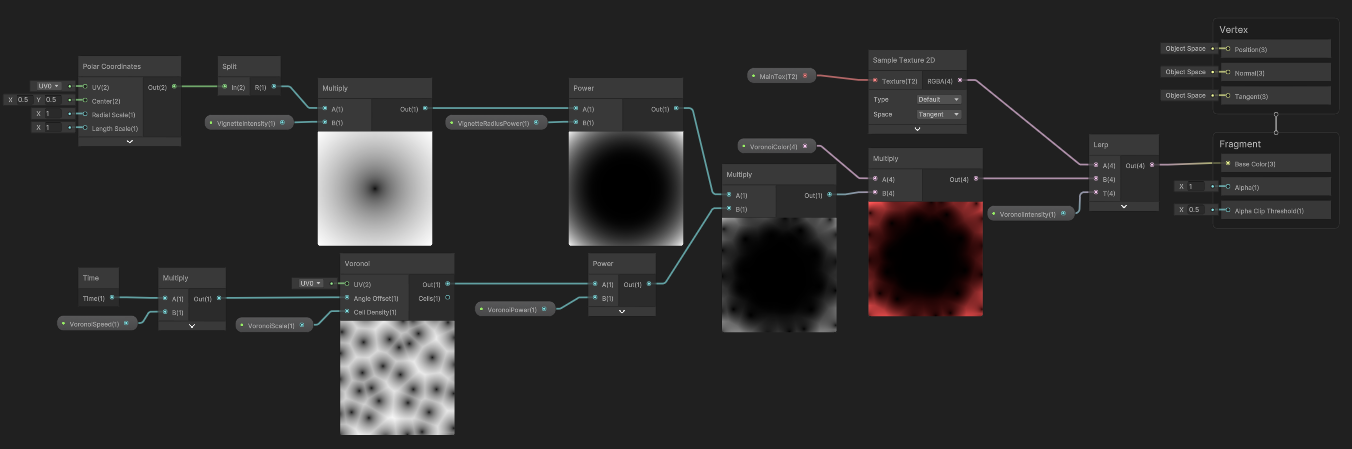
\includegraphics[width=1\linewidth]{Images/vignetteShader.png}
    \caption{Shader winiety odpowiedzialnej za wyświetlanie na ekranie gracza informacji o ilości utraconego życia}
\end{figure}
\begin{figure}[h]
    \centering
    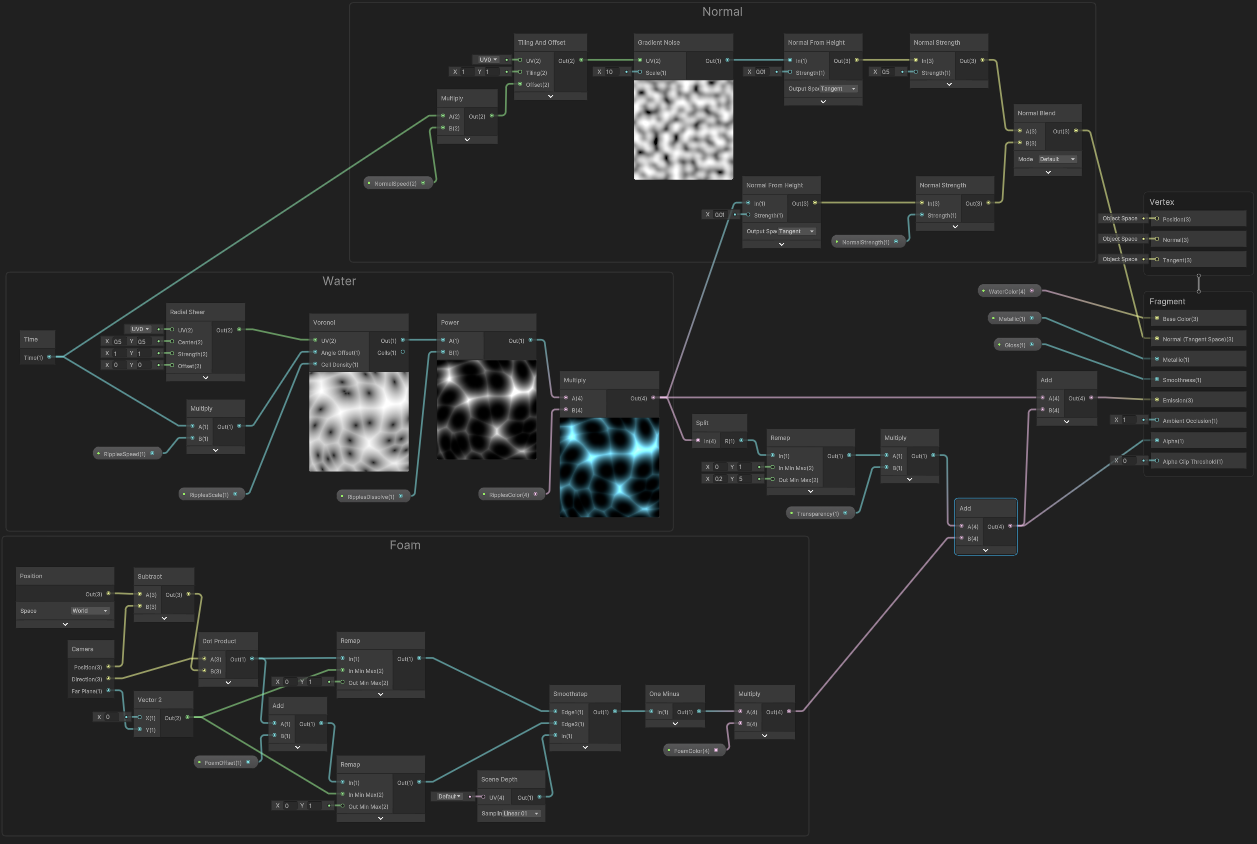
\includegraphics[width=1\linewidth]{Images/waterShader.png}
    \caption{Shader wody, którą znajdziemy w fontannie znajdującej się na terenie parku}   
\end{figure}
\begin{figure}[h]
    \centering
    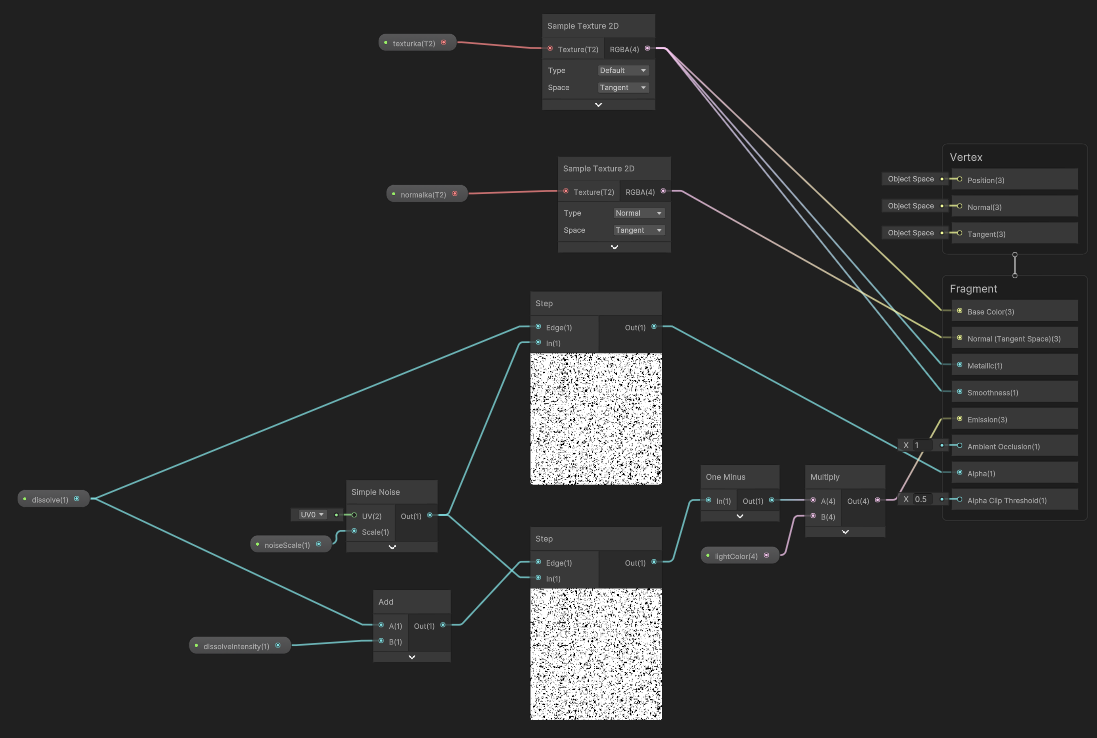
\includegraphics[width=1\linewidth]{Images/dissolve.png}
    \caption{Prostsza wersja shadera zanikania, używana w przypadku podniesienia interaktywnych obiektów takich jak kamizelka kuloodporna, apteczka czy granaty}
\end{figure}
\FloatBarrier